
\begin{figure}[!t]
    \centering
    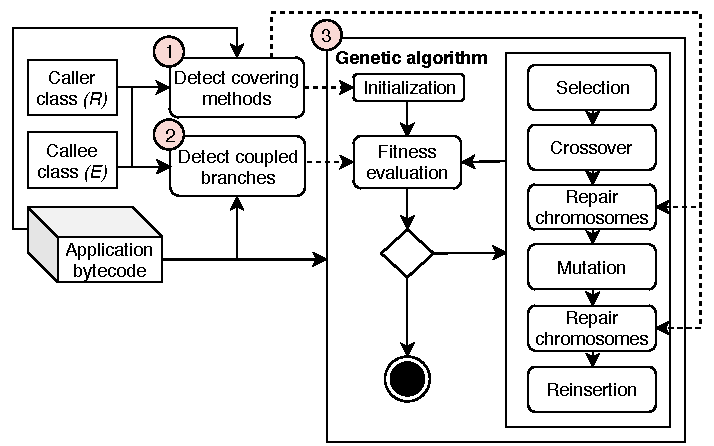
\includegraphics[width=\columnwidth]{papers/cling/figures/approach.pdf}
    \caption{General overview of \integration}
    \label{fig:cling:approach}
\end{figure}

The main idea of our \underline{cl}ass \underline{in}tegration testin\underline{g} (hereinafter referred to as \cling) is to test a class by leveraging its usage by another class.
More specifically, we focus on the calls between the former, the callee ($E$), and the latter, the caller ($R$). By doing so, we benefit from the additional context setup by $R$ before calling~$E$ (\eg initializing a complex input parameter), and the additional post-processing after $E$ returns (\eg using the return value later on in $R$), thus (implicitly) adding assertions on the behavior of $E$. 

Figure \ref{fig:cling:approach} presents the general overview of \cling. \cling takes as input a pair of caller-callee $\langle R,E \rangle$ classes with at least one call (denoted \textbf{call site} hereafter) from $R$ to $E$. Since the goal of \cling is to generate test cases covering $E$ by calling methods in $R$, the first step (\circled{1}) collects the list of \textit{covering methods} in $R$ that, when called, may directly or indirectly cover statements in $E$. This list is later used  during the generation process to ensure that test cases contain calls to covering methods. The second step (\circled{2}) analyzes the CCFGs of $R$ and $E$ to identify the coupled branches between $R$ and $E$ used later on to guide the search. Finally, the generation of the test cases  (\circled{3}) uses a genetic algorithm with two additional \textit{repair} steps, ensuring that the crossover and mutation only produce test cases able to cover lines in $E$. The result is a test suite for $E$, whose test cases invokes methods in $R$ that cover the interactions between $R$ and $E$.

The remainder of this section describes our novel underlying Coupled Branches Criterion, the corresponding search-heuristics, and test case generation in \cling. 

%This study focuses on the call coupling between a class pair. We indicate these two classes as \emph{caller class} and \emph{callee class}. The \emph{caller class} must have at least one call site to \emph{callee class} (denoted \textit{interesting call sites} hereafter). The goal of \integration is covering different paths in the CFG of a given \emph{callee class} through generating tests for another given class (\emph{caller class}). The rationale behind this approach is that the generated unit tests for \textit{callee class} can be improved by some extra tests which are leveraging the usages of \textit{callee class} by the other classes.

%The main steps of \integration are demonstrated in Figure \ref{fig:cling:approach}. Before starting the search process, this approach executes two processes: \textit{Detect covering methods} and \textit{Detect branches}.
%\textit{Detect covering methods} collects methods that calling them may lead to covering the statements of \textit{callee class} (indicated as \textbf{covering methods} hereafter), and passes them to the generation processes (initialization and repair chromosomes). Also, \textit{Detect branches} collects the list of interesting edges, in both of the \textit{caller class} and \textit{callee class}, for each \textit{interesting call site}. These interesting edges are used in determining search fitness functions.
%
%In this section, we explain our new test criterion and the fitness functions driving the test generation process. Then, we detail the different steps of our novel approach.

\begin{figure}[t]
	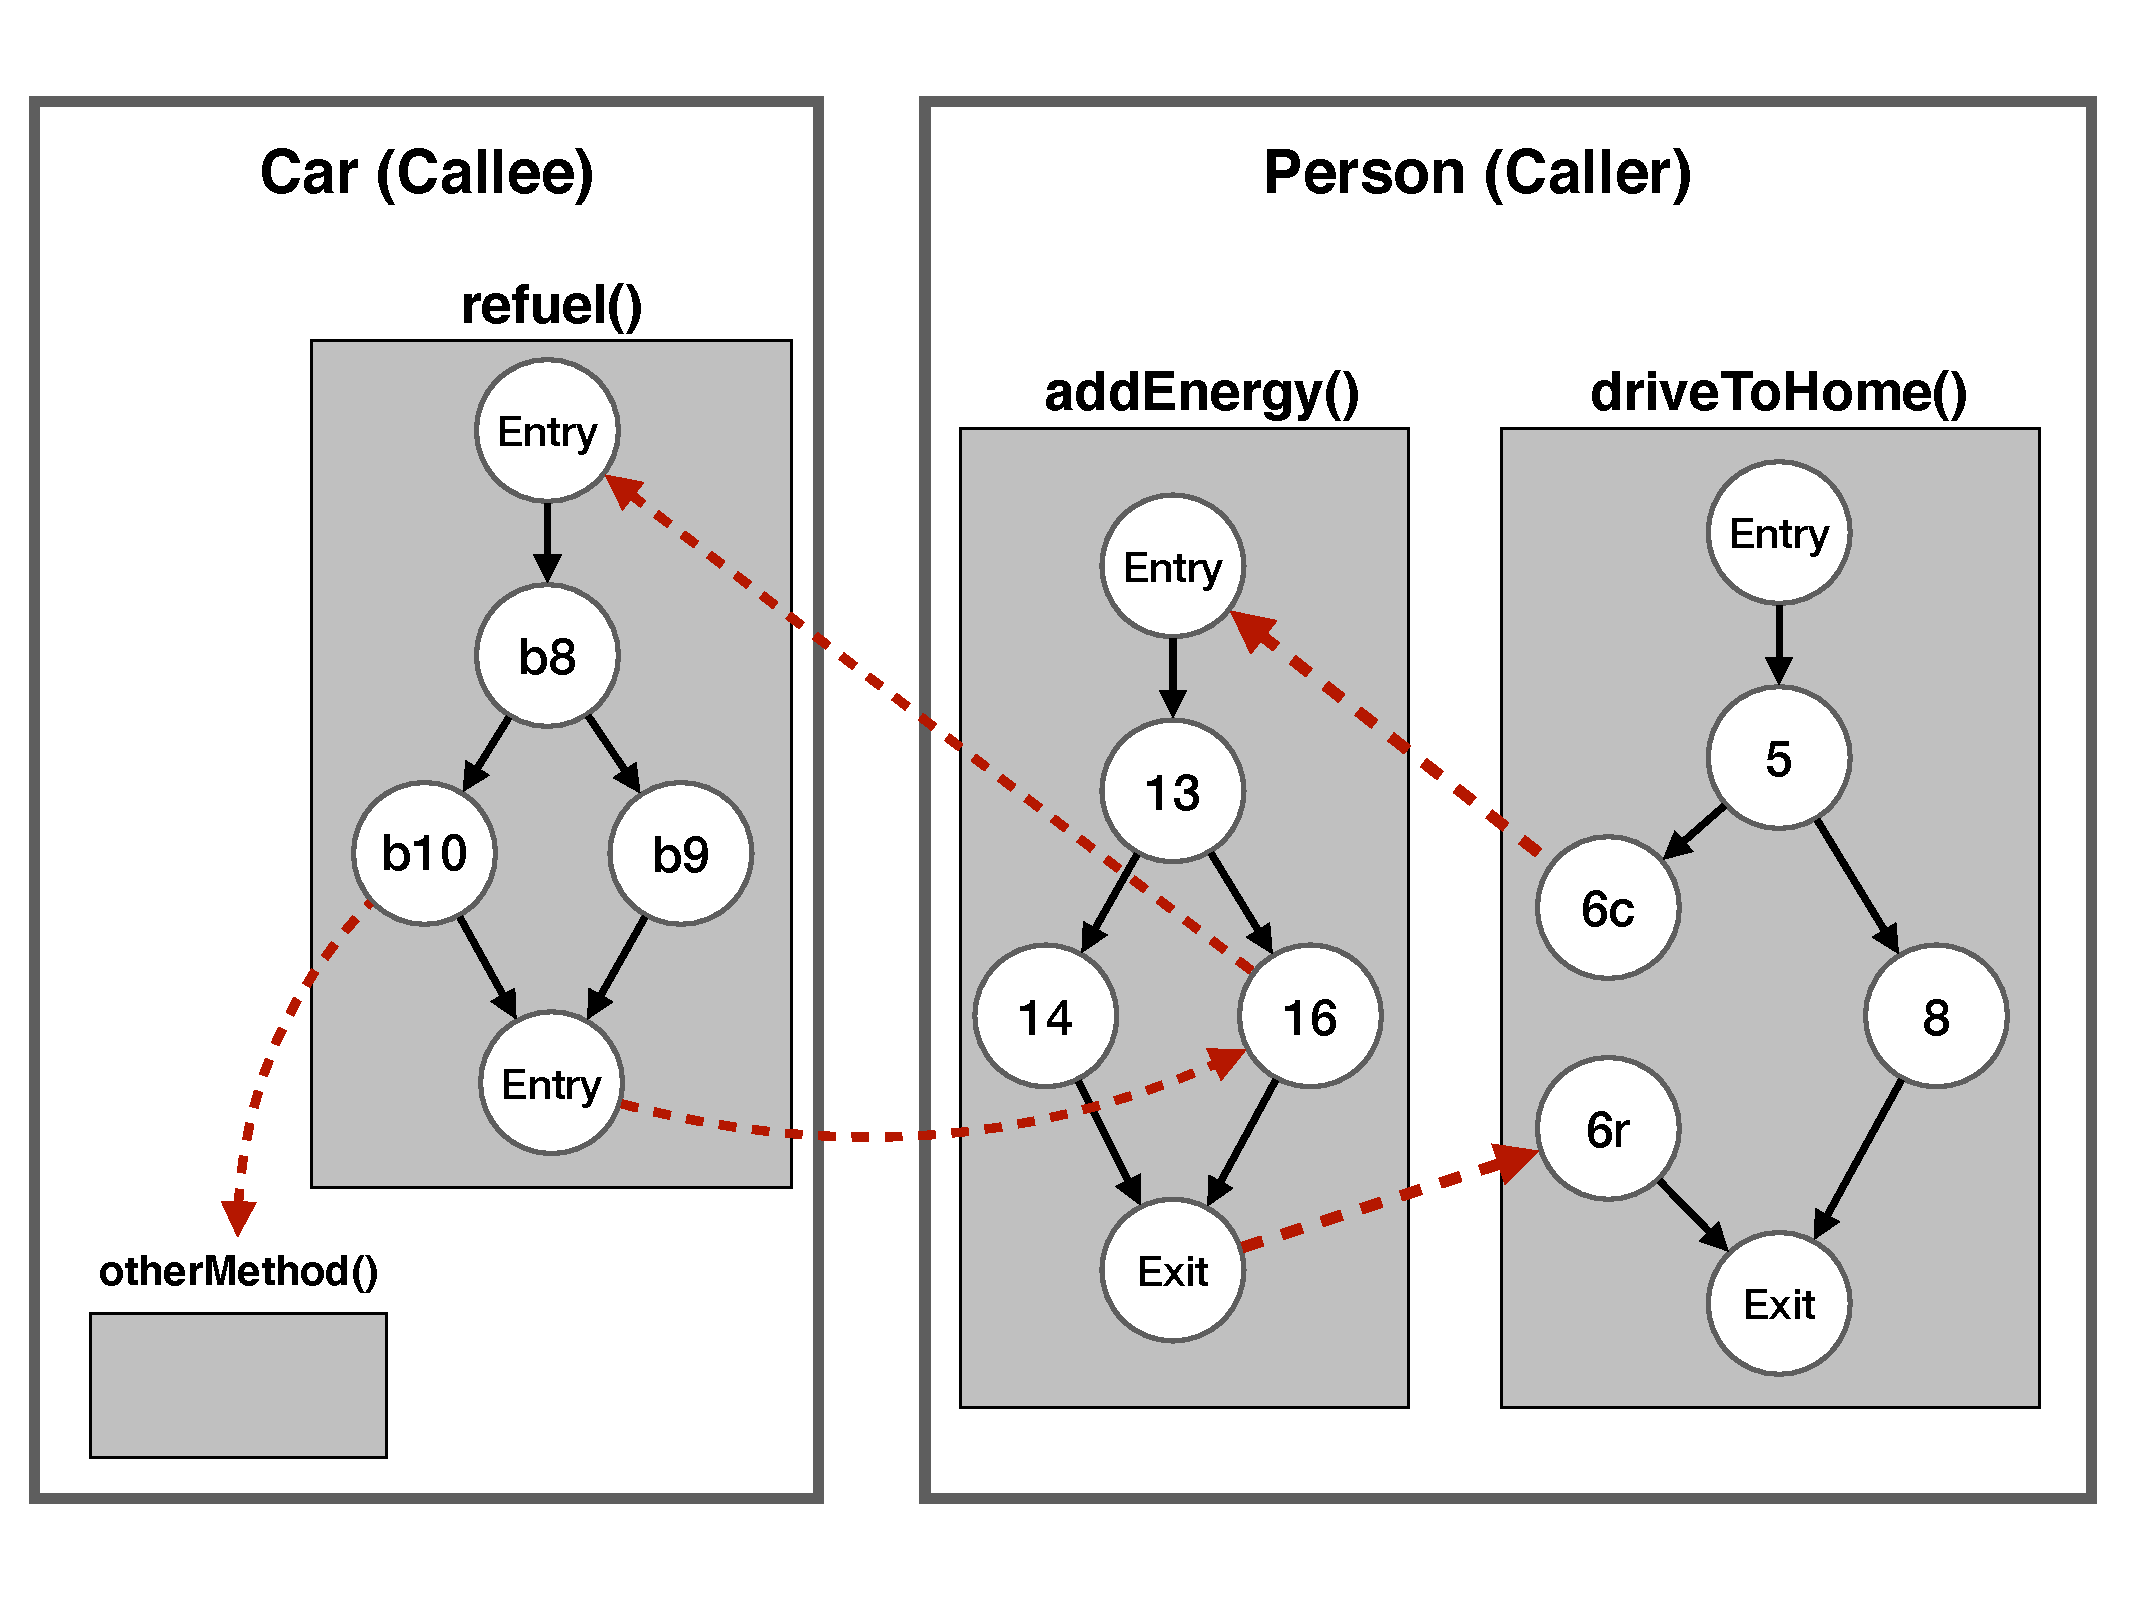
\includegraphics[width=1.0\linewidth]{papers/cling/figures/CCFG_merge}
	\caption{Merging CCFGs of two classes: \texttt{Person} (caller) and \texttt{Car} (callee)}
  \label{fig:CCFF_new}
\end{figure}




\subsection{Coupled Branch testing criterion}

%\subsubsection{Defining the Coupled Branches} 
\label{sec:approach:coupledBranchDef}

%\begin{figure}[t]
%    \centering
%    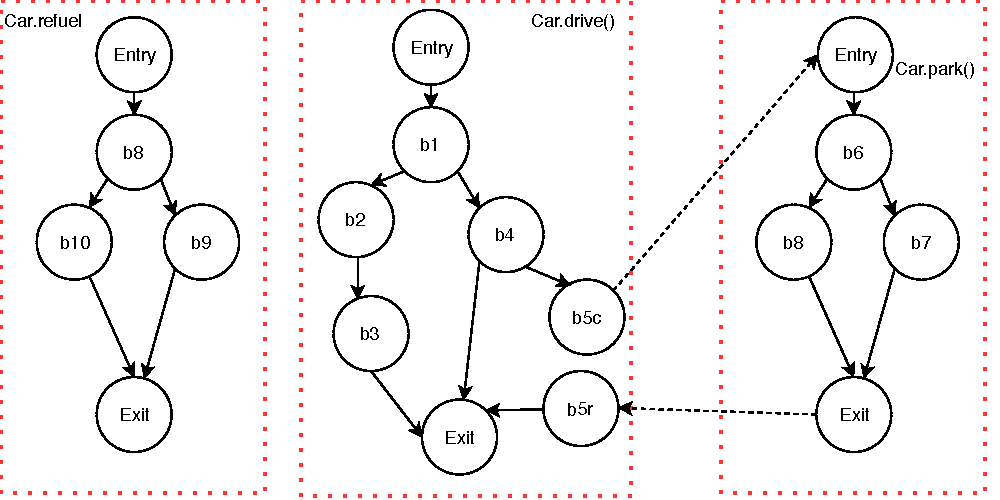
\includegraphics[width=\columnwidth]{figures/BCCFG.pdf}
%    \caption{Class control flow graph of class B}
%    \label{fig:bccfg}
%\end{figure}

%The coupled branch criterion can be used for testing a pair of classes (\textit{caller class} and \textit{callee class}). This criterion provides an opportunity to test various combinations of certain class pairs behaviors. Since this criterion only focuses on the call couplings between these two classes, it requires to test control flow paths in the CCFG of \textit{caller class}, which reaches to an interesting call site, with the paths in the CCFG of \textit{callee class}, which starts from the entry point of the called method in that call site and ends in one of the exit points of the CCFG. For detecting these paths, we detect the \textit{interesting edges} in each of these CCFGs.

To test the integration between two classes $E$ and $R$, we need to define a coverage criterion that helps us to measure how thoroughly a test suite $T$ exercises the interaction calls between the two classes ($E$ and $R$). One possible coverage criterion would consist of testing all possible paths (\textit{inter-class path coverage}) that start from the entry node of the caller $R$, execute the integration calls to $E$ and terminate in one of the exit points of $R$. However, such a criterion will be affected by the \textit{path explosion problem}~\cite{cadar2013symbolic}: the number of paths increases exponentially with the cyclomatic complexity of $E$ and $R$, and thus the number of interaction calls between the two classes.

%\andy{Seems CBC stands for ``Coupled Branch Criterion'' or ``Coupled Branches Criterion''... we should stick to 1?}
To avoid the \textit{path explosion problem}, we define an integration-level coverage criterion, namely the Coupled Branch Criterion (CBC), where the number of coverage targets remains polynomial to the cyclomatic complexity of $E$ and $R$. More precisely, CBC focuses on call coupling between caller and callee classes. Intuitively, let $s \in R$ be a call site, i.e., a call statement to a method of the class $E$. Our criterion requires to cover all pairs of branches $ (b_r, b_e)$, where $b_r$ is a branch in $R$ that leads to $s$ (the method call), and $b_e$ is a branch of the callee $E$ that is not trivially covered by every execution of $E$. So, in the worst case, the number of coverage targets is quadratic in number of branches in the caller and callee classes.


\subsubsection{Target caller branches}
Among all branches in the caller class, we are interested in covering the branches that, when executed, always lead to the integration call site (i.e., calling the callee class). We refer to these branches as \textit{target branches} for the caller.
To understand how we determine the target branches in the caller, 
% Before introducing the formal definition of the criterion, 
let us consider the example of the caller and the callee in Figure~\ref{fig:CCFF_new}. The code for the class \texttt{Person} is reported in Figure~\ref{list:cling:ClassA}. The class \texttt{Person} contains two methods, \texttt{addEnergy()} and \texttt{driveToHome()}, with the latter invoking the former (line 6 in Listing~\ref{list:cling:ClassA}). The method \texttt{Person.addEnergy()} invokes the method \texttt{refuel()} of the class \texttt{Car} (line 16 in Listing~\ref{list:cling:ClassA}). The method \texttt{Person.driveToHome()} invokes the method \texttt{Car.drive()} (line 8 in Listing~\ref{list:cling:ClassA}). Therefore, the class \textit{Person} is the caller, while \texttt{Car} is the callee. 

Figure~\ref{fig:CCFF_new} shows an excerpt of the Class-level Control Flow Graphs (CCFGs) for the two classes. In the figure, the names of the nodes are labelled with the line number of the corresponding statements in the code of Listing~\ref{list:cling:ClassA}. Node 16 in \texttt{Person.addEnergy()} is a call site to \texttt{Car.refuel()}; it is also control dependent on nodes 5 (\texttt{Person.driveToHome()}) and 13 (\texttt{Person.addEnergy()}). Furthermore, node 16 only post-dominates branch $\langle 13,16\rangle$. Instead, the branch $\langle 5,6c\rangle$ is not post-dominated by  node 16 as covering $\langle 5,6c\rangle$ does not always imply covering node 16 as well. Therefore, the branches in the caller \texttt{Person.addEnergy()} that always lead to the callee are $B_{\mathtt{Person}}(\mathtt{Car.refuel()})=\{\langle 13,16\rangle\}$. 
%%
Hence, among all branches in the caller class (\texttt{Person} in our example), we are interested in covering the branches that, when executed, always lead to the integration call site (i.e., calling the callee class). We refer to these branches as \textit{target branches} for the caller.
 
% Considering that $CCFG_{Caller}$ is the CCFG of \textit{caller class}. The \textit{interesting} edges of interesting call site $Ics$ in this graph should have two conditions:
% \begin{inparaenum}[(i)]
%    \item it should be among the outgoing edges of nodes on which $Ics$ is control dependent; and
%    \item $Ics$ should dominate the edge.
%\end{inparaenum}
%The formal definition of interesting edges, in \textit{caller class}, for interesting call site $Ics$ is presented in Equation \ref{eq:caller_side_branches}:
%
%
%\begin{equation} \label{eq:caller_side_branches}
%    %
%    \begin{split}
%    IECaller_{Ics} = \{x : x \in E_{Caller} \wedge Pd(Ics,x) \wedge tail(x) \in CDN_{Ics}\}
%    %
%    \end{split}
%\end{equation}
%Where $E_{Caller}$ is the set of edges in $CCFG_{Caller}$; $CDN_n$ is the set of nodes on which $n$ is control dependent in graph $CCFG_{Caller}$; $Pd(n,e)$ indicates if node $n$ post dominates edge $e$; and $tail(e)$ is the tail of edge $e$ in $CCFG_{Caller}$.
\begin{definition}[\textit{Target branches for the caller}]
\textit{For a call site $s$ in $R$, the set of target branches $B_{R}(s)$ for the caller $R$ contains the branches having the following characteristics:
 \begin{inparaenum}[(i)]
    \item the branches are outgoing edges for the node on which $s$ is control dependent (\ie nodes for which $s$ post-dominates one of its outgoing branches but does not post-dominate the node itself); and
    \item the branches are post-dominated by $s$ (\ie branches for which all the paths through the branch to the exit point pass through $s$).
\end{inparaenum}
}
\end{definition}

%
%For instance, if the class \texttt{Person} in Figure \ref{list:ClassA} is the caller class and the class \texttt{Car} in Figure \ref{fig:bccfg} is the callee class. For the call site to \texttt{Car.refuel()} in node 20, node 20 is control dependent on nodes 9 and 17 but only post-dominates branch $<17,20>$, so $B_{\mathtt{Person}}(\mathtt{Car.refuel()}) = \{<17,20>\}$.

%\xavier{Can someone double check the example above? I think there was a mistake in the original one (commented below) because branch $<9,10c>$ is not post-dominated by the call site. There is a path that avoids the call site in the CCFG.}

%As we can see in Figures \ref{fig:refuelCar} and \ref{fig:takeBus}, nodes 12 and 20 are the interesting call sites. 
%These interesting call sites are control dependent on node 9 and nodes 9 and 17, respectively. Among the outgoing edges of node 9, First interesting call site (node 12) only post-dominates edge $<9,12>$. So, this edge is the only edge in set $IECaller_{12}$. Similarly, the other call site (node 20) post-dominates edges $<9,10c>$ (from outgoing edges of node 9) and $<17,20>$ (from outgoing edges of node 17). Hence, this edge is the only edge in set $IECaller_{20}$.

%Assuming that $CCFG_{Callee}$ is CCFG of \textit{callee class}. 
%The interesting edges of interesting edge $Ics$ in this graph should have two conditions:
% \begin{inparaenum}[(i)]
% \item They should be among the outgoing edges of branching nodes (nodes which has more than one outgoing edge); and 
% \item \emph they should be accessible from the entry node of the called method in $Ics$.
%\end{inparaenum}
%The formulation of interesting edges, in \textit{callee class}, for interesting call site $Ics$ is demonstrated in Equation \ref{eq:callee_side_branches}:
%
%\begin{equation} \label{eq:callee_side_branches}
%    %
%    \begin{split}
%        IECallee_{Ics} = \{x : x \in E_{Callee} \wedge |O(tail(x))| > 1 \\ 
%        \wedge \ A_{CCFG_{Callee}}(EN_{Ics},x)\}
%    \end{split}
%    %
%\end{equation}
%
%Where $EN_{Ics}$ is the entry node of called method in $Ics$; $E_{Callee}$ is the set of edges in $CCFG_{Callee}$; function $A_G(N_1,N_2)$ indicates if node $N_2$ is accessible from node $N_1$ in control flow graph $G$; and $OE(N)$ is the set of outgoing edges from node $N$.

%\andy{Do we consider it an issue that the code listing for Car is not in the paper?}
\subsubsection{Target callee branches}
Let us consider the example of Figure~\ref{fig:CCFF_new}  again. This time, let us look at the branches in the callee (\texttt{Car}) that are directly related to the integration call. In the example, executing the method call  \texttt{Car.refuel()} (node 16 of the method \texttt{Person.addEnergy()}) leads to the execution of the branching node $b8$ of the class \texttt{Car}. Hence, the set of branches affected by the interaction calls is $B_{\mathtt{Car}}(\mathtt{Car.refu}$-$\mathtt{el()}) = \{\langle b8,b9\rangle;$ $\langle b8,b10\rangle\}$. In the following, we refer to these branches as \textit{target branches} for the callee. Note that, for a call site $s$ in $R$ calling $E$, the set of target branches for the callee also  includes branches that are trivially executed by any execution of $s$. 

\begin{definition}[\textit{Target branches for the callee}]
\textit{
The set of target branches $B_{E}(s)$ for the caller $E$ contains branches satisfying the following properties: \begin{inparaenum}[(i)]
 \item the branches are among the outgoing branches of branching nodes (\ie the nodes having more than one outgoing edge); and 
 \item the branches are accessible from the entry node of the method called in $s$.
\end{inparaenum}
}
\end{definition}

%In our example, the called methods of class $Car$ (callee class) by class $Person$ (caller class) are $Car.drive()$ and $Car.refuel()$. As it demonstrated by Figure \ref{fig:bccfg}, the accessible branching nodes from the entry nodes are $b1$, $b4$, and $b6$ for $Car.drive()$ and $b8$ for $Car.refuel()$. So, the interesting edges for node 12 ($IECallee_{12}$), which calls $Car.drive()$, are outgoing edges of nodes $b1$ and $b4$: $<b1,b2>, <b1,b4>, <b4,Exit>, <b4,b5c>,<b6,b7>$, and $<b6,b8>$. In the same manner, the interesting edges for node 20 ($IECallee_{20}$), which calls $Car.refuel()$, are outgoing edges of node $b8$:  $<b8,b9>$ and $<b8,b10>$.
\subsubsection{Coupled branches}
Given the sets of target branches for both the caller and  callee, an integration test case should exercise at least one target branch for the caller (branch affecting the integration call) and one target branch for the callee (i.e., the integration call should lead to covering branches in the callee). In the following, we define pairs of target branches $(b_r \in B_{R}(s), b_e \in B_{E}(s))$ as \textit{coupled branches} because covering  $b_r$ can lead to covering $b_e$ as well. In our example of Figure~\ref{fig:CCFF_new}, we have two coupled branches: the branches $(\langle 13,16\rangle,\langle b8,b9\rangle)$ and the branches $(\langle 13,16\rangle$, $\langle b8,b10\rangle)$.

\begin{definition}[\textit{Coupled branches}]
\textit{
Let $B_{R}(s)$ be the set of target branches in the caller class $R$; let $B_{E}(s)$ be the set of target branches in the callee class $E$; and let $s$ be the call site in $R$ to the methods of $E$. The set of coupled branches $CB_{R,E}(s)$ is the cartesian product of $B_{R}(s)$ and $B_{E}(s)$:
}
\begin{equation}\label{def2}
	CB_{R,E}(s) = CB_{R,E}(s) = B_{R}(s) \times B_{E}(s)
\end{equation}
\end{definition}
%The set of \emph{coupled branches} $CB_{R,E}(s)$ for a call site $s$ from $R$ to $E$ is the product of $B_{R}(s)$ by  $B_{E}(s)$: $CB_{R,E}(s) = B_{R}(s) \times B_{E}(s)$.  

\begin{definition}\label{def3}
\textit{
Let $S=(s_1, \dots, s_k)$ be the list of call sites from a caller $R$ to a callee $E$, the set of coupled branches for $R$ and $E$ is the union of the coupled branches for the different call sites $S$: $CB_{R,E} = \cup_{s \in S} CB_{R,E}(s)$.
}
\end{definition}

%The \textit{Coupled Branches} of each interesting call site $Ics$ is the set of edge pairs which are made by combining edges in $IECaller_{Ics}$ and $IECallee_{Ics}$.
%The \textit{Coupled Branches} set is formalized in Equation \ref{eq:coupled_branches}:
%
%\begin{equation} \label{eq:coupled_branches}
%    \begin{split}
%    Coupled\_Branches_{Ics} = IECaller_{Ics} \times IECallee_{Ics}
%    \end{split}
%\end{equation}
%
%Where function $EN(m)$ gives the entry node of CFG of method $m$; $cm_x$ is the called method in call site $x$; $A_{CCFG_{Caller}}(b_1,x)$ indicates that call site $x$ is accessible from edge $e_1$ in $CCFG_{Caller}$; and $A_{CCFG_{Callee}}(EN(cm_x),e_2)$ evalauates the accesibility of edge $e_2$ from the entry node of the called method in call site $x$.
%
%In our example, as we described, node 12 is one of the interesting call sites. Its coupled branches ($Coupled\_Branches_{12}$) is the combination of edges in $IECaller_{12}$ and $IECallee_{12}$. This set contains $1 \times 6 = 6$ edge pairs. Also, the coupled branches of our second interesting call site ($Coupled\_Branches_{20}$) is the combination of edges in $IECaller_{20}$ and $IECallee_{20}$. This set contains $2 \times 2 = 4$ edge pairs.

%The set of coupled branches for a given caller and callee class is the union of the \textit{coupled branches} of the interesting call sites. The formalized definition of coupled branches of \textit{caller class} $C_1$ and \textit{callee class} $C_2$ is presented in Equation \ref{eq:coupled_branches_classes}.
%
%\begin{equation} \label{eq:coupled_branches_classes}
%    \begin{split}
%    CB_{C_1, C_2} = \{\bigcup\limits_{Ics \in I(C_1,C_2)}  Coupled\_Branches_{Ics} \}
%    \end{split}
%\end{equation}
%Where $I(C_1,C_2)$ gives the set of interesting call sites between caller class $C_1$ and callee class $C_2$.
%
%In our example, $CB_{Person, Car}$ is the union of sets $Coupled\_Branches_{12}$ and $Coupled\_Branches_{20}$.

\subsubsection{Coupled Branches Criterion (CBC)}\label{sec:approach:coupledBranchCrit}

%This criterion requires that the test suite \textit{T} covers all of the edge pairs which are indicated as coupled branches of a particular caller class and callee class. \textit{T} covers an edge pair if this test set contains at list one test case which covers both of these edges.

% Assuming that $T= \{ t_1, t_2, ..., t_n\}$ is a test suite which contains $n$ test cases. And, we want to check CBC for classes $C_1$, as the \textit{caller class}, and $C_2$ as the \textit{callee class}. Also, $I$ is the set of interesting call sites between these two classes. In this case, $T$ fulfills CBC if it coveres all of the edge pairs which are indidicated as coupled branches of call sites in $I$. This definition is formalized in Equation \ref{eq:cbc}:

% \begin{equation} \label{eq:cbc}
%     \begin{split}
%         \forall Ics \in I: \forall (e_1,e_2) \in Coupled\_Branches_{Ics} : \\
%          \exists t \in T : t \  covers \ e_1 \wedge t \ covers \ e_2
%     \end{split}
% \end{equation}

%To measure CBC of a test suite $T= \{ t_1, t_2, ..., t_n\}$ for \textit{caller class} $C_1$ and \textit{callee class} $C_2$, we use Equation \ref{eq:cbc-measure}. This equation is representing the percentage of covered \textit{coupled branches} of these two classes.
%
%\begin{equation} \label{eq:cbc-measure}
%    \begin{split}
%        \frac{|{(e_1,e_2): (e_1,e_2) \in CB_{C_1, C_2} \wedge (\exists t \in T: t \ covers \ e_1 \ and \ e_2)}|}{|CB_{C_1, C_2}|}
%    \end{split}
%\end{equation}
%
%Where $(e_n,e_m)$ is an edge pair in the \textit{coupled branches} of the given classes.
Based on the definition above, the CBC criterion requires that for all the call sites $S$ from a caller $R$ to a callee $E$, a given test suite $T$ covers all the coupled branches:
$$
CBC_{R,E} = \frac{
        \vert \{(r_i,e_i) \in CB_{R,E} \vert \exists t \in T: t \ covers \ r_i \ and \ e_i\} \vert
    }{
        \vert CB_{R,E} \vert
    }
$$
%
%As for classical branch pair coverage, achieving $100 \%$ is not always possible because the conditions in the branching nodes are in a specific situation that covering both of the edges in the edge pair is not possible. Detecting and filterin these kind of branch pairs are not easy as they need some expensive symbolic executions.
%
We do note that this formula is only relevant if there are indeed call interactions between caller and callee.
As for classical branch and branch-pair coverage, $CB_{R,E}$ may contain unreachable branch-pairs. However, detecting and filtering those incompatible pairs is an undecidable problem. Hence, in this study, we target all coupled branches.
\subsubsection{Inheritance and polymorphism}
\label{subsec:inheritance}

\begin{lstlisting}[frame=tb,
    caption={Class GreenPerson},
    label=list:ClassAPrime,
    captionpos=t,
    numbers=left,
    belowskip=-2em,
    float=t,
    language=java,
    firstnumber=1]
Class GreenPerson extends Person{
    private HybridCar car = new HybridCar();
    @override
    public void addEnergy(){
        if(this.lazy){
            takeBus();
        }else if (chargerAvailable()){
            car.recharge()
        }else{
            car.refuel();
        }
    }

    private void chargerAvailable(){
        if(ChargingStation.takeavailableStations().size > 0){
            return true;
        }
        return false;
    }
}
\end{lstlisting}

%Assuming the given \textit{caller class} and {callee class} are in the same inheritance tree. In this case, one of the classes is \textit{superclass} and the other one is a \textit{subclass} which extends \textit{superclass}. To support polymorphism by introduced criterion, we use a different procedure for finding the call sites and generating CCFG of given classes.

%A call site from a \textit{superclass} to a \textit{subclass} is the basic blocks which have a call to one of the overridden methods by \textit{subclass}. Also, a call site from a \textit{subclass} to a \textit{superclass} is the basic blocks having a call to one of the declared methods in the \textit{superclass} which is not overridden by \textit{subclass}.
  
%The CCFG of a \textit{superclass} is made by merging the CFGs of the methods which are defined in the \textit{superclass} but not overridden by \textit{subclass}. Furthermore, the CCFG of a \textit{subclass} is composed by merging the CFGs of the methods which are particularly defined or overridden by \textit{subclass}. Hence, the CFGs of inherited methods from \textit{superclass} which is not overridden by \textit{subclass} is not merged into this CCFG.

In the special case where the caller and callee classes are in the same inheritance tree, we use a different procedure to build the CCFG of the super-class and find the call sites $S$. The CCFG of the super-class is built by merging the CFGs of the methods that are not overridden by the sub-class. As previously, the CCFG of the sub-class is built by merging the CFGs of the methods defined in this class, including the inherited methods overridden by the sub-class (other non-overridden inherited methods are not part of the CCFG of the sub-class).

%As an illustration, consider that class $GreenPerson$ (Listing \ref{list:ClassAPrime}) extends class $Person$. This class represents a person who has a hybrid car. So, for adding energy to her car, she can either refuel or recharge her car (lines 7 to 11). This class overrides method $addEnergy()$ from its superclass. Also, it declares a new method named $chargerAvailable()$ which indicates if the charging station is available or it is occupied.

%As demonstrated in Figure \ref{fig:subSuperClasses}, the CFG of method $addEnergy()$ is not used in the composition of $Person$ CCFG (Figure \ref{fig:personAsSuperCCFG}). In this graph, nodes $10$ and $28-29$, which call to an overridden method, are call sites to $GreenPerson$.
% Morover, we only use the CFG of overriden method $addEnergy()$ and newly defined method $chargerAvailable()$ for creating CCFG of $GreenPerson$ (Figure \ref{fig:greenPersonCCFG}), and we do not use the other inherited methods (methods $driveToHome ()$ and $takeBus ()$) in this CCFG. In this graph node $6$, which calls a non-overriden inherited method, is call site to $Person$.

For instance, the class \texttt{GreenPerson} in Listing \ref{list:ClassAPrime}, representing owners of hybrid cars, extends class \texttt{Person} from Listing \ref{list:cling:ClassA}. For adding energy, a green person can either refuel or recharge her car (lines 7 to 11). \texttt{Green\-Person} overrides the method \texttt{Person.add\-En\-er\-gy()} and defines an additional method \texttt{Green\-Person.char\-ger\-Avai\-la\-ble()} indicating whether the charging station is available. Only those two methods are used in the CCFG of the class \texttt{Green\-Person} presented in Figure \ref{fig:greenPersonCCFG}, inherited methods are not included in the CCFG; the CCFG of the super-class \texttt{Person} does not contain the method \texttt{Person.addEnergy()}, redefined by the sub-class \texttt{GreenPerson}.

The call sites $S$ are identified according to the CCFGs, depending on the caller and the callee. If the caller $R$ is the super-class, $S$ will contain all the calls in $R$ to methods that have been redefined by the sub-class. For instance, nodes 6 and 13 in Figure \ref{fig:CCFF_new} with \texttt{Person} as caller. If the caller $R$ is the sub-class, $S$ will contain all the calls in $R$ to methods that have been inherited but not redefined by $R$. For instance, node 6 in Figure \ref{fig:greenPersonCCFG} with \texttt{GreenPerson} as caller.

\begin{figure}[!t]
  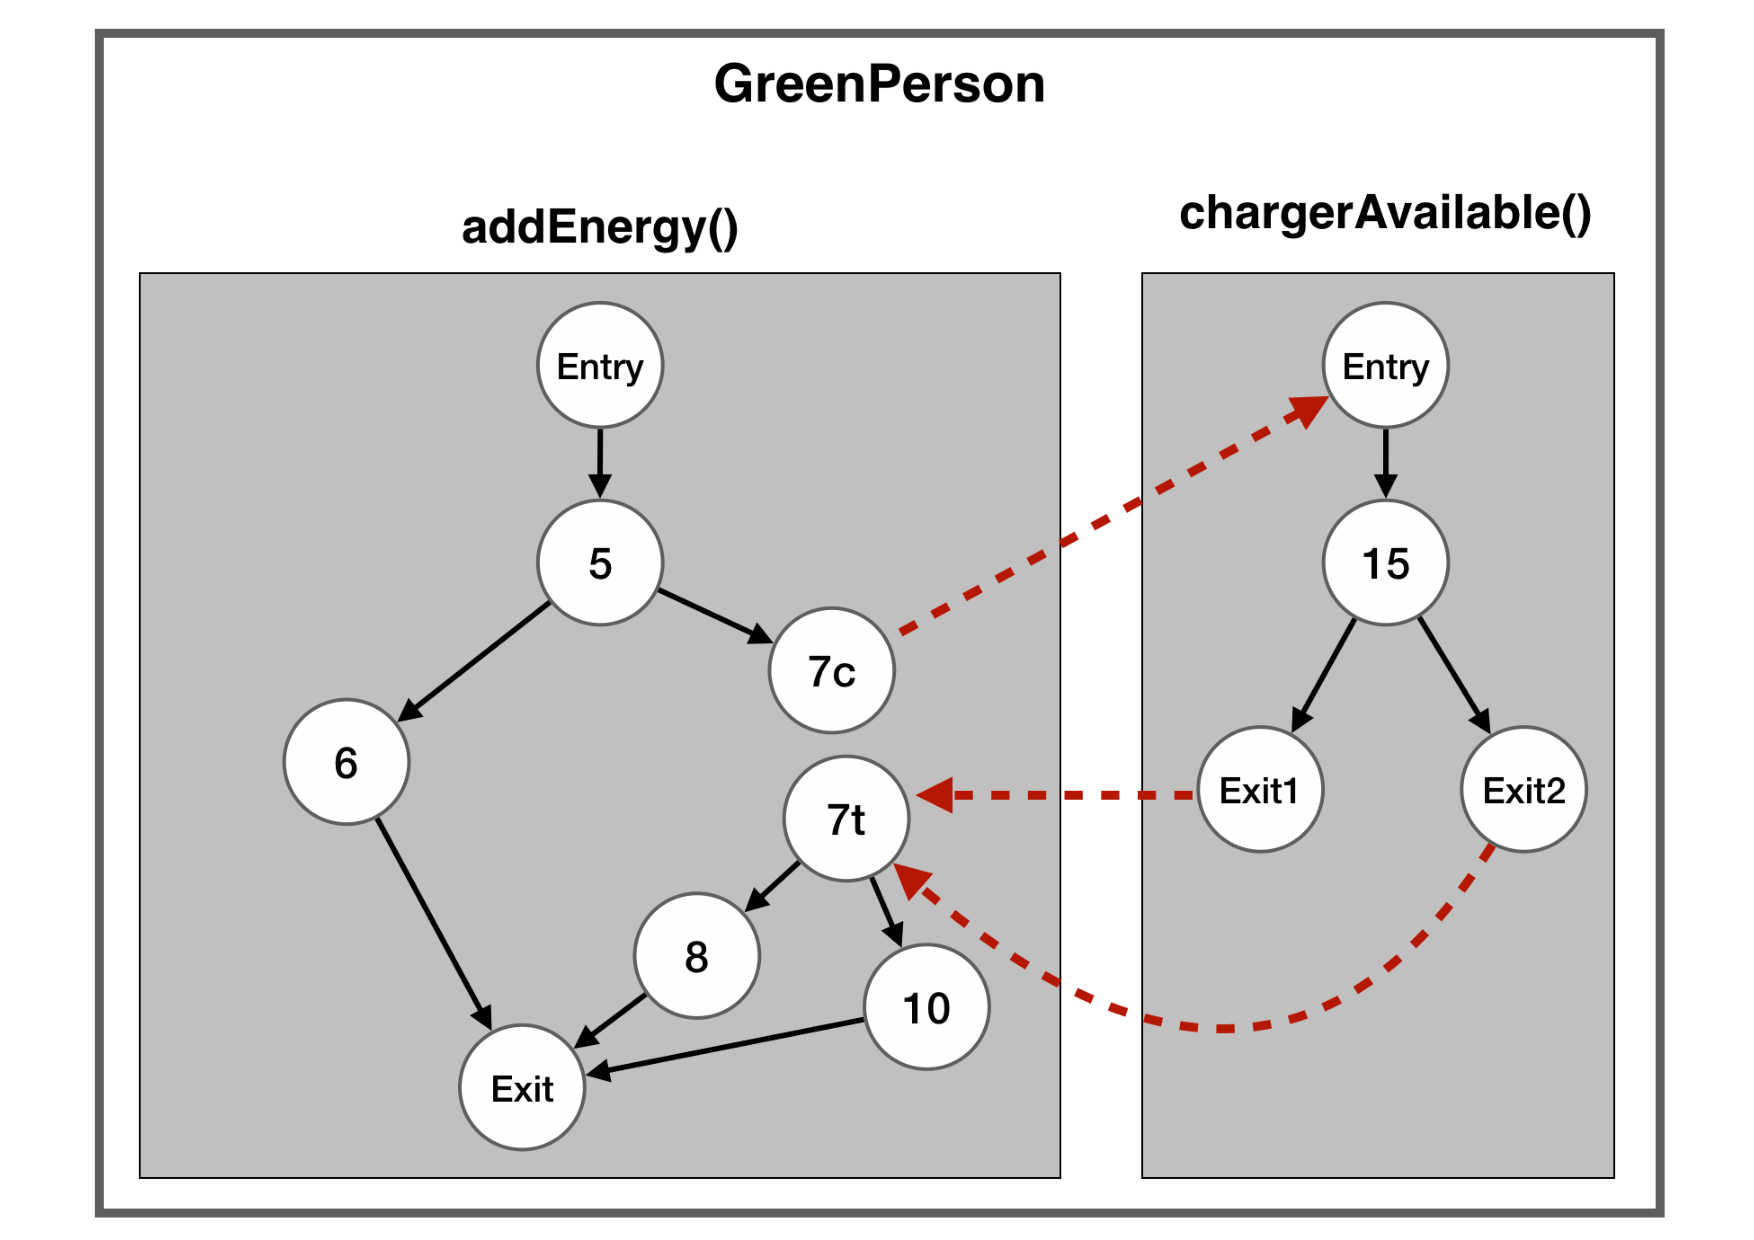
\includegraphics[width=0.98\linewidth]{papers/cling/figures/GreenPerson2}
\caption{CCFG of $GreenPerson$ as subclass}
\label{fig:greenPersonCCFG}
\end{figure}
 

\subsubsection{Advantage of using CBC}
Prior works proposed to use dataflow based criteria for integration testing~\cite{Jin1998, Harrold1994,Alexander2000, Alexander2003, Alexander2004, Alexander2010}. Hence, in this section, we discuss the advantages of using CBC compared to these criteria.
CBC does not construct dataflow graphs and, consequently, calculates the coverage targets faster. CBC also requires covering additional interactions between caller and callee compared to the other criteria relying on dataflow graphs to indicate the coupling paths. As an example, assume a variable \textit{v1} defined by \textit{node 13} in method \texttt{addEnergy()} of class \texttt{Person} (Figure \ref{fig:CCFF_new}), and that is used afterward by \textit{node b8} in method \texttt{refuel()} of class \texttt{Car} to decide whether the next step of the execution is \textit{node b9} or \textit{b10}. In this scenario, even if we choose a criterion to cover all of the independent paths between the definition (\textit{node 13}) and usage (\textit{node b8}) of the variable, it does not require to cover both outgoing branches of \textit{b8} ($\langle b8,b9\rangle$ and $\langle b8,b10\rangle$). However, depending on the way that  \textit{v1} is defined in node \textit{b8}, the execution may cover outgoing branches of \textit{b8}. In contrast, CBC requires covering all of the target branches in the \texttt{Person} class with both of these two branches in the \texttt{Car} class. 

 %%%%%%%%%%%%%%%%%%%%%
\subsection{\cling}
\label{sec:cling}
 %%%%%%%%%%%%%%%%%%%%%

%\integration gets \emph{application's bytecode}, \emph{caller class}, and \emph{callee class} as input.
%Then, it leverages evolutionary-based approaches to generate a test suite which
%tests callee through caller class. The main goal of this approach is to generate a test suite satisfying the CBC criterion.
\cling is the tool that we have developed to generate integration-level test suites that maximize the proposed CBC adequacy criterion. The inputs of \cling are the (1) \emph{application's bytecode}, (2) a \emph{caller class} $R$, and (3) \emph{callee class} $E$. As presented in Figure \ref{fig:cling:approach}, \cling first detects the covering methods (step \circled{1}) and identifies the coupled branches $CB_{R,E}(s)$ for the different call sites (step \circled{2}), before starting the search-based test case generation process (detailed in the following subsections). \cling produces a test suite that maximizes the CBC criterion for $R$ and $E$.

%Figure \ref{fig:cling:approach} presents the main steps of this approach. First, \integration analyzes the bytecode of the caller class to detect the  \textit{interesting call sites class}. Next, it uses the definition provided in Section \ref{sec:approach:coupledBranchDef} to collect the coupled branches for each these call sites.
%In addition to coupled branches, \integration collects the \emph{covering methods} in caller class.
%A \emph{callable} method is a public or protected method that executing it leads to, at least, one interesting call site. We do note that a covering method does not contain an interesting call site. Its inner calls to the other methods of the class may have the call site. These detected \emph{covering methods} are passed to the search process. After collecting this information, the search starts. This process stops either when the assigned budget is passed or when the best-generated test suite covers all of the coupled branches.

% Since the only way that a test can reach to a callee class through caller class is the interesting call sites, \emph{covering methods}
% The reason that we pass the \emph{callable} methods to the search process is that

% This strategy assures that the generated test can even execute a call site in a private method. The test generation process in \integration has higher priority for using \emph{covering methods}. 
% This prioritization gives a higher chance to the randomly generated test cases for testing a path which passes from an external call site to \textit{callee class}. 

%In the following sections, we outline more details the search process and the fitness function it uses in \integration.

%\subsubsection{Genetic algorithm}

%Existing search-based software testing approaches use a single-objective, multi-objective, or many-objective optimisation algorithms. In single-objective approaches, all of the targets are aggregated into a single fitness function. On the contrary, multi and many-objective approaches contain more than one fitness function and try to reach all of them at a time. The difference between those two approaches is that multi-objective can accept up to three fitness functions, but many-objective is capable of handling even more objectives.

Satisfying the CBC criterion is essentially a many-objective problem where integration-level test cases have to cover pairs of coupled branches separately. In other words, each pair of coupled branches corresponds to a search objective to optimize. The next subsection describes our search objectives.

\subsubsection{Search objectives}
In our approach, each objective function measures the distance of a generated test from covering one of the coupled branch pairs. The value ranges between $[0,+\infty)$ (zero denoting that the objective is satisfied).
Assuming that $CB_{R,E} = \{c_1, c_2, \ldots, c_n \}$ is the set of coupled branches $\langle r_i, e_i \rangle$ between $R$ and $E$. Then, the fitness for a test case $t$ is defined as follows: 

%
% \begin{equation} \label{eq:fitness_functions}
    % \begin{numcases}
    %   d(c_1,t) = D(r_1,t) + D(e_1,t)\\
    %   ... \\
    %   d(c_n,t) = D(r_n,t) + D(e_n,t)\\
    % \end{numcases}
% \end{equation}
% %


\rowcolors{1}{}{}
\begin{equation}\label{eq:fitness_functions}
    Objectives = \left\{
    \begin{array}{lcr}
        d(c_1,t) = D(r_1,t) + D(e_1,t)\\
        \dots\\
        d(c_n,t) = D(r_n,t) + D(e_n,t)\\
    \end{array}
    \right.
\end{equation}
\rowcolors{1}{}{gray!15}

\noindent where $D(b,t) = al(b,t) + bd(b,t) $ computes the distance between the test $t$ to the branch $b$ using the classical approach level $al(b,t)$ and normalized branch distance $bd(b,t)$ \cite{McMinn2004}.

\subsubsection{Test Case Generation}
To solve such a many-objective problem, we tailored the Many-Objective Sorting Algorithm (MOSA)~\cite{Panichella2015} to generate test cases through class integration. MOSA has been introduced and assessed in the context of unit test generation~\cite{Panichella2015} and security testing~\cite{jan2019search}. Besides, previous studies \cite{Campos2018, Panichella2015} showed that MOSA is very competitive compared with alternative algorithms when handling hundreds and thousands of testing objectives. Interested readers can find more details about the original MOSA algorithm in Panichella \etal~\cite{Panichella2015}. Although a more efficient variant of MOSA has been recently proposed~\cite{Panichella2018}, such a variant (DynaMOSA) requires to have a hierarchy of dependencies between coverage targets that exists only at the unit level. Since targets in unit testing are all available in the same control flow graph, the dependencies between objectives can be calculated (\ie control dependencies). In contrast, \cling's objective is covering combinations of targets in different control flow graphs. Since covering one combination does not depend on the coverage of another combination, DynaMosa is not applicable to this problem.

% This approach saves all of the test cases satisfying at least one of the goals to an \emph{archive}. The final test suite is made from this \emph{archive}. Also, MOSA focuses the search process to the goals which are not covered yet.
Therefore, in \integration, we tailored MOSA to work at integration level, targeting pairs of coupled branches rather than unit-level coverage targets (e.g., statements). In the following, we describe the main modifications we applied to MOSA to generate integration-level test cases.
 
% \begin{equation} \label{eq:distance}
%    D(b,t) = al(b,t) + bd(b,t) \\
%\end{equation}
%
%In this equation, $al(b,t)$ is the approach level which indicates the number of control dependent edges between the closest executed edge by test $t$ and edge $b$. $bd(b,t)$ is the normalized branch distance of the closest executed control dependent branch (by test case $t$) to edge $b$.

\subsubsection{Initial population}
The search process starts by generating an initial population of test cases. A random test case is a sequence of statements (\textit{object instantiations}, \textit{primitive statements}, \textit{method calls}, and \textit{constructor calls to the class under test}) of variable lengths. More precisely, the random test cases include \textit{method calls} and \textit{constructors} for the caller $R$, which directly or indirectly invoke methods of the callee $E$ (\textit{covering methods}). Although \integration generates these test cases randomly, it extends the initialization procedure used for search-based crash reproduction \cite{soltani2017}. In particular, the initialization procedure in \cling gives a higher priority to methods in the caller class $R$ that invoke methods of the callee class $E$. While calls to other methods of $R$ are also inserted, their insertion has a lower probability. This prioritization ensures to generate tests covering call sites to the callee class. In the original MOSA algorithm, all methods of the class under test are inserted in each random test case with the same probability without any prioritization.

% \begin{algorithm}
% \DontPrintSemicolon
% \SetKwInOut{Input}{input}  
% \Input{Set of public and protected methods in caller class $C$\\
% Set of detected covering methods $M$\\
% Population size $N$\\
% maximum size of the genrated test case $MAX\_SIZE$
% }
%     \KwResult{A set of test cases $P_0$, $|P_0| = N$}
%     \Begin{
%       $P_0 \longleftarrow \emptyset$\;
%       $used\_calls \longleftarrow \emptyset$\;
%         \nl\While{$|P_0| < N$}{\label{code:big_while_start}
%         $t \longleftarrow$ empty test case\;\label{code:empty_test}
%         $tSize \longleftarrow$ random integer $\in [1:MAX\_SIZE]$\;\label{code:test_size}
%         $insert\_probability \longleftarrow$$1 / tSize$\;
%         % \nlset{REM} remove $x$ from the list of $T$ of maximal index\;\label{InResR}
%         \While{$t.size() <  tSize$}{\label{code:inner_while_start}
%           \eIf{$ random\_number \le  insert\_probability $}{
%             \If{$|M| == 0$}{\label{code:insert_callable_start}
%                 $M \longleftarrow used\_calls$\;
%                 $used\_calls \longleftarrow emptyset$\;
%             }\label{code:refill_end}
%             $call \longleftarrow$ choose randomly from $M$\;

%             $M \longleftarrow M - call$\;\label{code:remove_from_M}
%             $used\_calls \longleftarrow used\_calls \cup call$\;\label{code:add_to_used}
            
%             $insert\_probability \longleftarrow$$1 / tSize$\;\label{code:insert_callable_end}
%             }{
%                 $call \longleftarrow$ choose randomly from $C$\;\label{code:insert_random_start}
%                 $length \longleftarrow t.size()$\;
%                 $insert\_probability \longleftarrow 1 / (tSize-length+1)$\;\label{code:insert_random_end}
%             }

%             Insert $call$ to test $t$\;
%           }\label{code:inner_while_end}
%           $P_0 \longleftarrow P_0 \cup t$\;\label{code:add_test_to_population}
%         }\label{code:big_while_end}
%       }
%     \caption{Initialize the first population}\label{alg:initial_population}
%     \end{algorithm}

%For initializing the first population, we use the algorithm proposed by Soltani \etal \cite{soltani2017}. The focus of this initialization algorithm is a target method which is appeared in the given stack trace. This algorithm generates a random test case for the initial population. Then, it adds the target method to the test case with a probability. The only difference in our algorithm is that we have different target methods (the detected \textit{covering methods}). So, each time, we randomly add one of these methods to the randomly generated test cases.

% Algorithm \ref{alg:initial_population} shows the applied algorithm for generating the initial population. This algorithm requires as input \begin{inparaenum}[(i)]
%         \item the set of the public and protected method calls in the given caller class $C$, 
%         \item covering methods detected before starting the search process $M$, 
%         \item the population size $N$, and
%         \item the maximum statements that an individual test case can have $MAX\_SIZE$.
% \end{inparaenum}
% Each iteration on loop in lines \ref{code:big_while_start} to \ref{code:big_while_end} generates a new random test case for the initial population. In this loop, first, we make an empty test case (line \ref{code:empty_test}). Then, we set the size of this test ($tSize$) (line \ref{code:test_size}). This size varies between 1 to the given $MAX\_SIZE$. Accordingly, the probability of inserting a detectable method to the test is adjusted according to this size (line 8).

% The loop in lines \ref{code:inner_while_start} to \ref{code:inner_while_end} randomly inserts method calls from $C$ or $M$ to the test case: in each iteration, according to the covering methods insertion probability $insert\_probability$, we add a method from either $M$ (lines \ref{code:insert_callable_start} to \ref{code:insert_callable_end}) or from $C$ (lines \ref{code:insert_random_start} to \ref{code:insert_random_end}). The value of this probability is low at the beginning ($1/tSize$). However, it increases with any insertion from $C$ (line \ref{code:insert_random_end}). in the worst case, if the algorithm adds all of the methods from $C$, the value of this value of this probability reaches to $1$ in the last iteration. Hence, this algorithm ensures that each test case contains at least one covering method from $M$. Moreover, when we select a covering method for insertion, algorithm removes it from $M$ and puts it in the $used\_calls$ (lines \ref{code:remove_from_M} and \ref{code:add_to_used}). When algorithm uses all of the covering methods in $M$, we refill this set and clear the $used\_calls$ (line \ref{code:insert_callable_start} to \ref{code:refill_end}). With this procedure, we make sure that the generated tests in the initial population contain a diverse population of the covering methods.

% Finally each generated test case is added to the initial population $P_0$ (Line \ref{code:add_test_to_population}).

\subsubsection{Mutation and crossover}\label{sec:mutation_and_crossover} \cling uses the traditional single-point crossover and mutation operators (adding, changing and removing  statements) \cite{Fraser2011} with an additional procedure to repair broken chromosomes. The initial test cases are guaranteed to contain at least one \textit{covering method} (a method of $R$ that directly or indirectly invokes methods of $E$). However, mutation and crossover can lead to generating \textit{offspring} tests that do not include any \textit{covering method}. We refer to these chromosomes as \textit{broken chromosomes}. To fix the broken chromosomes, the \textit{repair procedure} works in two different ways, depending on whether the broken chromosome is created by the crossover or by the mutation. 

If the broken chromosome is the result of the mutation operator, then the repair procedure works as follows: let $t$ be the broken chromosome and let $M$ be the list of covering methods; then, \cling applies the mutation operator to $t$ in an attempt to insert one of the covering methods in $M$. If the insertion is not successful, then the mutation operator is invoked again within a loop. The loop terminates when either a covering method is successfully injected in $t$ or when the number of unsuccessful attempts is greater than a threshold ($50$ by default). In the latter case, $t$ is not inserted in the new population for the next generation.

If the broken chromosome is generated by the crossover operator then the broken child is replaced by one of its parents.
%This additional procedure ensures that the test cases still contain calls to the covering methods (\ie still executes code able to cover the callee) after application of the operators. By replacing one of the children by its parent for the single-point crossover operator; or by applying additional mutations (with a maximum of 50 additional mutations) to try to reinsert a call to one of the covering methods for the other mutation operators. 

%\begin{algorithm}
%    \DontPrintSemicolon
%    \SetKwInOut{Input}{input}  
%    \Input{
%        Set of detected covering methods $M$\\
%    Chromosomes before corssover $Parent_1, Parent_2$\\
%    Chromosomes after corssover $Child_1, Child_2$\\
%    }
%        \KwResult{A pair of repaired chromosomes $RC_1, RC_2$}
%        \Begin{
%            \eIf{$Child_1$ contains a method from $M$}{\label{code:child1_check_start}
%                $RC_1 \longleftarrow Child_1$\;\label{code:child1_is_repaired}
%                }{
%                $RC_1 \longleftarrow Parent_1$\;\label{code:parent1_is_repaired}
%                }
%
%                \eIf{$Child_2$ contains a method from $M$}{\label{code:child2_check_start}
%                $RC_2 \longleftarrow Child_2$\;
%                }{
%                $RC_2 \longleftarrow Parent_2$\;
%                }\label{code:child2_check_end}
%          }
%        \caption{Repairing chromosomes after crossover}\label{alg:crossover_repair}
%        \end{algorithm}
%
%
%        \begin{algorithm}
%            \DontPrintSemicolon
%            \SetKwInOut{Input}{input}  
%            \Input{
%                Set of detected covering methods $M$\\
%            Mutated chromosome $mutated$\\
%            }
%                \KwResult{Repaired mutated chromosome $RC$}
%                \Begin{
%                    $nTries \longleftarrow 0$\;
%                    \While{$mutated$ does not contain a method from $M$\\
%                    $\&\&\:\: nTries \le 50$}{\label{code:mutation_loop_start}
%                        $RANDOM\_MUTATION(mutated)$\;\label{code:mutate-again}
%                        $nTries++$;\
%                    }\label{code:mutation_loop_end}
%                    $RC \longleftarrow mutated$\;
%                  }
%                \caption{Repairing chromosomes after mutation}\label{alg:mutation_repair}
%                \end{algorithm}
%\subsubsection{Repairing broken chromosomes}
%
%As discussed in the previous sections, the search process in \integration focuses on the \text{covering methods}. Since it is possible that the genetic operators modify the tests in a way that they lose their call to the covering methods, we have a procedure to repair the chromosomes after each of these operators. This repairing process makes sure that the search process keeps a higher priority for the covering methods in the next iterations of the search process.
%
%Algorithm \ref{alg:crossover_repair} details the repairing process after the single-point crossover operator. This operator gets two tests (parents) from the existing population and selects and exchanges their statements to create two offsprings. In this scenario, it is possible that one of the offsprings misses all of the statements which invoke a covering method. Hence, to avoid this situation, our repairing process gets the parents pair ($Parent_1$ and $Parent_2$), as well as the set of covering methods $M$, and their offsprings ($Child_1$ and $Child_2$). Then, it checks if $Child_1$ contains any method from $M$ (Line \ref{code:child1_check_start}). If this test contains any covering method, the chromosome does not need repair ( Line \ref{code:child1_is_repaired}). On the contrary, if it does not have any \textit{covering method}, the algorithm passes its parent ($Parent_1$) as the repaired chromosome (Line \ref{code:parent1_is_repaired}). Next, we repeat the same process for $Child_2$ (Lines \ref{code:child2_check_start} to \ref{code:child2_check_end}).
%
%Missing the \textit{covering method} can occur during the mutation as well as removing one or more statements is part of the test mutation. Consequently, there is a low probability that the mutated test misses its calls to the \textit{covering methods}. In this case, our repairing process, iteratively, mutates the chromosome and checks if any covering method is added.
%
%Algorithm \ref{alg:mutation_repair} highlights the main steps of this repairing process. This algorithm gets the detected covering methods $M$ and the mutated chromosome $mutated$. If $mutated$ contains any covering method, it does not need any repair. On the contrary, if it loses the method, the algorithm enters into the loop in lines \ref{code:mutation_loop_start} to \ref{code:mutation_loop_end}. In this loop, we mutate the $mutated$ test again (Line \ref{code:mutate-again}) and check if the method is attached. If any \textit{covering method} is added to $mutated$, the algorithm stops the iteration and pass the test as the repaired chromosome. To avoid the infinite loop, we put a limit for the number of mutations. If the algorithm reaches to the maximum number of allowed mutations (50), it stops the iteration and passes the $mutated$ test, which is mutated 50 times, as the repaired chromosome.

\subsubsection{Polymorphism}
\label{sec:approach:polymorphism}

%If \integration gets a pair of super/subclass as the input, it follows the same procedure. The only difference is in the scenario that the given \textit{caller class} is the superclass. In this situation, we cannot generate tests for \textit{caller class} and expect coverage on the \textit{callee class} because the initialized object is the superclass and we do not have defined methods by subclass (\textit{callee class}).
%In this particular case, we generate tests for \textit{callee class}, but we select the covering methods from the ones which are used for the composition of superclass CCFG. With this slight change, we can expect to cover the coupled branches defined between CCFG of superclass and subclass.

If the caller and callee are in the same hierarchy and the caller is the super-class, \cling cannot generate tests for the caller class that will cover the callee class (since the methods to cover are not defined in the super-class). 
This is the case for instance if the super-class (caller) calls abstract methods defined in the sub-class (callee).
In this particular case, \cling generates tests for the callee class. However, it selects the covering methods only from the inherited methods which are not overridden by the callee (sub-class). A covering method should be able to cover calls to the methods that have been redefined by the sub-class. With this slight change, \cling can improve the CBC coverage, as described in Section \ref{subsec:inheritance}.

